\documentclass[12pt]{scrartcl}

\setlength{\parindent}{0pt}
\setlength{\parskip}{.25cm}

\usepackage{graphicx}

\usepackage{xcolor}

\definecolor{darkred}{rgb}{0.5,0,0}
\definecolor{darkgreen}{rgb}{0,0.5,0}
\usepackage{hyperref}
\hypersetup{
  letterpaper,
  colorlinks,
  linkcolor=red,
  citecolor=darkgreen,
  menucolor=darkred,
  urlcolor=blue,
  pdfpagemode=none,
  pdftitle={CSCE 155E - Lab 1.0},
  pdfkeywords={}
}

\definecolor{MyDarkBlue}{rgb}{0,0.08,0.45}
\definecolor{MyDarkRed}{rgb}{0.45,0.08,0}
\definecolor{MyDarkGreen}{rgb}{0.08,0.45,0.08}

\definecolor{mintedBackground}{rgb}{0.95,0.95,0.95}
\definecolor{mintedInlineBackground}{rgb}{.90,.90,1}

%\usepackage{newfloat}
\usepackage[newfloat=true]{minted}
\setminted{mathescape,
               linenos,
               autogobble,
               frame=none,
               framesep=2mm,
               framerule=0.4pt,
               %label=foo,
               xleftmargin=2em,
               xrightmargin=0em,
               startinline=true,  %PHP only, allow it to omit the PHP Tags *** with this option, variables using dollar sign in comments are treated as latex math
               numbersep=10pt, %gap between line numbers and start of line
               style=default, %syntax highlighting style, default is "default"
               			    %gallery: http://help.farbox.com/pygments.html
			    	    %list available: pygmentize -L styles
               bgcolor=mintedBackground} %prevents breaking across pages
               
\setmintedinline{bgcolor={mintedBackground}}
\setminted[text]{bgcolor={mintedBackground},linenos=false,autogobble,xleftmargin=1em}
%\setminted[php]{bgcolor=mintedBackgroundPHP} %startinline=True}
\SetupFloatingEnvironment{listing}{name=Code Sample}
\SetupFloatingEnvironment{listing}{listname=List of Code Samples}

\title{CSCE 155 - C}
\subtitle{Lab 1.0 - Introduction\\
Online Version}
\author{Dr.\ Chris Bourke}
\date{~}

\begin{document}

\maketitle

\section*{Prior to Lab}

In each lab there may be pre-lab activities that you are 
\emph{required} to complete prior to attending lab.  Failure 
to do so may mean that you are not prepared to complete the
lab.  

\begin{enumerate}
  \item For this lab, you'll need to sign up with GitHub, a website
that hosts \emph{software repositories} using git (a distributed
version control system).  With GitHub you'll be able to store,
manage and backup your source code.  Git is an essential software
development tool that you'll want to fully utilize.  

Go to \url{https://github.com} and sign up using your 
\mintinline{text}{@huskers.unl.edu} email address so that GitHub 
will recognize you as a student.  This makes you eligible for
a lot of free software and other access.  After you have signed
up, you can get the GitHub Student Developer Pack at 
\url{https://education.github.com/pack} (but it is not necessary 
to complete this lab or for the course).

\item Claim your CSE account.  Your CSE account allows you to login
to the cse server and will be used to hand stuff in and to grade
yourself using the webgrader.  To claim your account go to 
\url{https://cse-apps.unl.edu/amu/claim} and follow the instructions
provided.  
\end{enumerate}


Some other department and university computing resources
and policies can be found at the following:

\begin{itemize}
  \item CSE Website: \url{http://cse.unl.edu}
  \item UNL Computing Policy: \url{http://www.unl.edu/ucomm/compuse/}
   \item CSE Academic Integrity Policy: \url{http://cse.unl.edu/academic-integrity-policy}
   \item CSE System Frequently Asked Questions (FAQ): \url{http://cse.unl.edu/faq}
   \item Account Management: \url{https://cse-apps.unl.edu/amu/}
   \item CSE Undergraduate Advising Page: \url{http://cse.unl.edu/advising}
   \item CSE Student Resource Center: \url{http://cse.unl.edu/src}
\end{itemize}

\section*{Peer Programming Pair-Up}

%TODO: consider additional edits to this section

\textbf{For students in the online section:} you may complete
the lab on your own if you wish or you may team up with a partner
of your choosing, or, you may consult with a lab instructor to get
teamed up online (via Zoom).

\textbf{For students in the face-to-face section:} your
lab instructor will team you up with a partner.  

To encourage collaboration and a team environment, labs are be
structured in a \emph{peer programming} setup.  At the start of
each lab, you will be randomly paired up with another student 
(conflicts such as absences will be dealt with by the lab instructor).
One of you will be designated the \emph{driver} and the other
the \emph{navigator}.  

The navigator will be responsible for reading the instructions and
telling the driver what to do next.  The driver will be in charge of the
keyboard and workstation.  Both driver and navigator are responsible
for suggesting fixes and solutions together.  Neither the navigator
nor the driver is ``in charge.''  Beyond your immediate pairing, you
are encouraged to help and interact and with other pairs in the lab.

Each week you should alternate: if you were a driver last week, 
be a navigator next, etc.  Resolve any issues (you were both drivers
last week) within your pair.  Ask the lab instructor to resolve issues
only when you cannot come to a consensus.  

Because of the peer programming setup of labs, it is absolutely 
essential that you complete any pre-lab activities and familiarize
yourself with the handouts prior to coming to lab.  Failure to do
so will negatively impact your ability to collaborate and work with 
others which may mean that you will not be able to complete the
lab.  

\section{Lab Objectives \& Topics}
At the end of this lab you should be familiar with the following
\begin{itemize}
  \item The CS50 IDE that you'll use for this course
  \item Basic unix commands
  \item Retrieving lab code from Github
  \item Modifying, compiling and executing your first C program
  \item Using CSE's web handin and web grader
\end{itemize}

\section{Activities}

\subsection{Getting Started}

Let's get started.  In order to develop programs in C you'll need
a code editor (plain text editor), a compiler (to compile the C code
into executable machine code) and a runtime environment (to actually
execute the program).  To do this, we'll run through how to use the 
CS50 Online IDE (Integrated Development Environment) developed by 
Harvard.  This is a web browser-based IDE that means you don't have
to install any software.  It is free and you login using your GitHub
account.  It also offers a \emph{persistent} environment: files you 
save or \emph{persist} in the IDE and be available next time you login.

Point your browser to the CS50 website and Sign in with GitHub:

\url{https://ide.cs50.io/}

Once logged in, it should looks something like the following.

\begin{figure}[h]
\centering
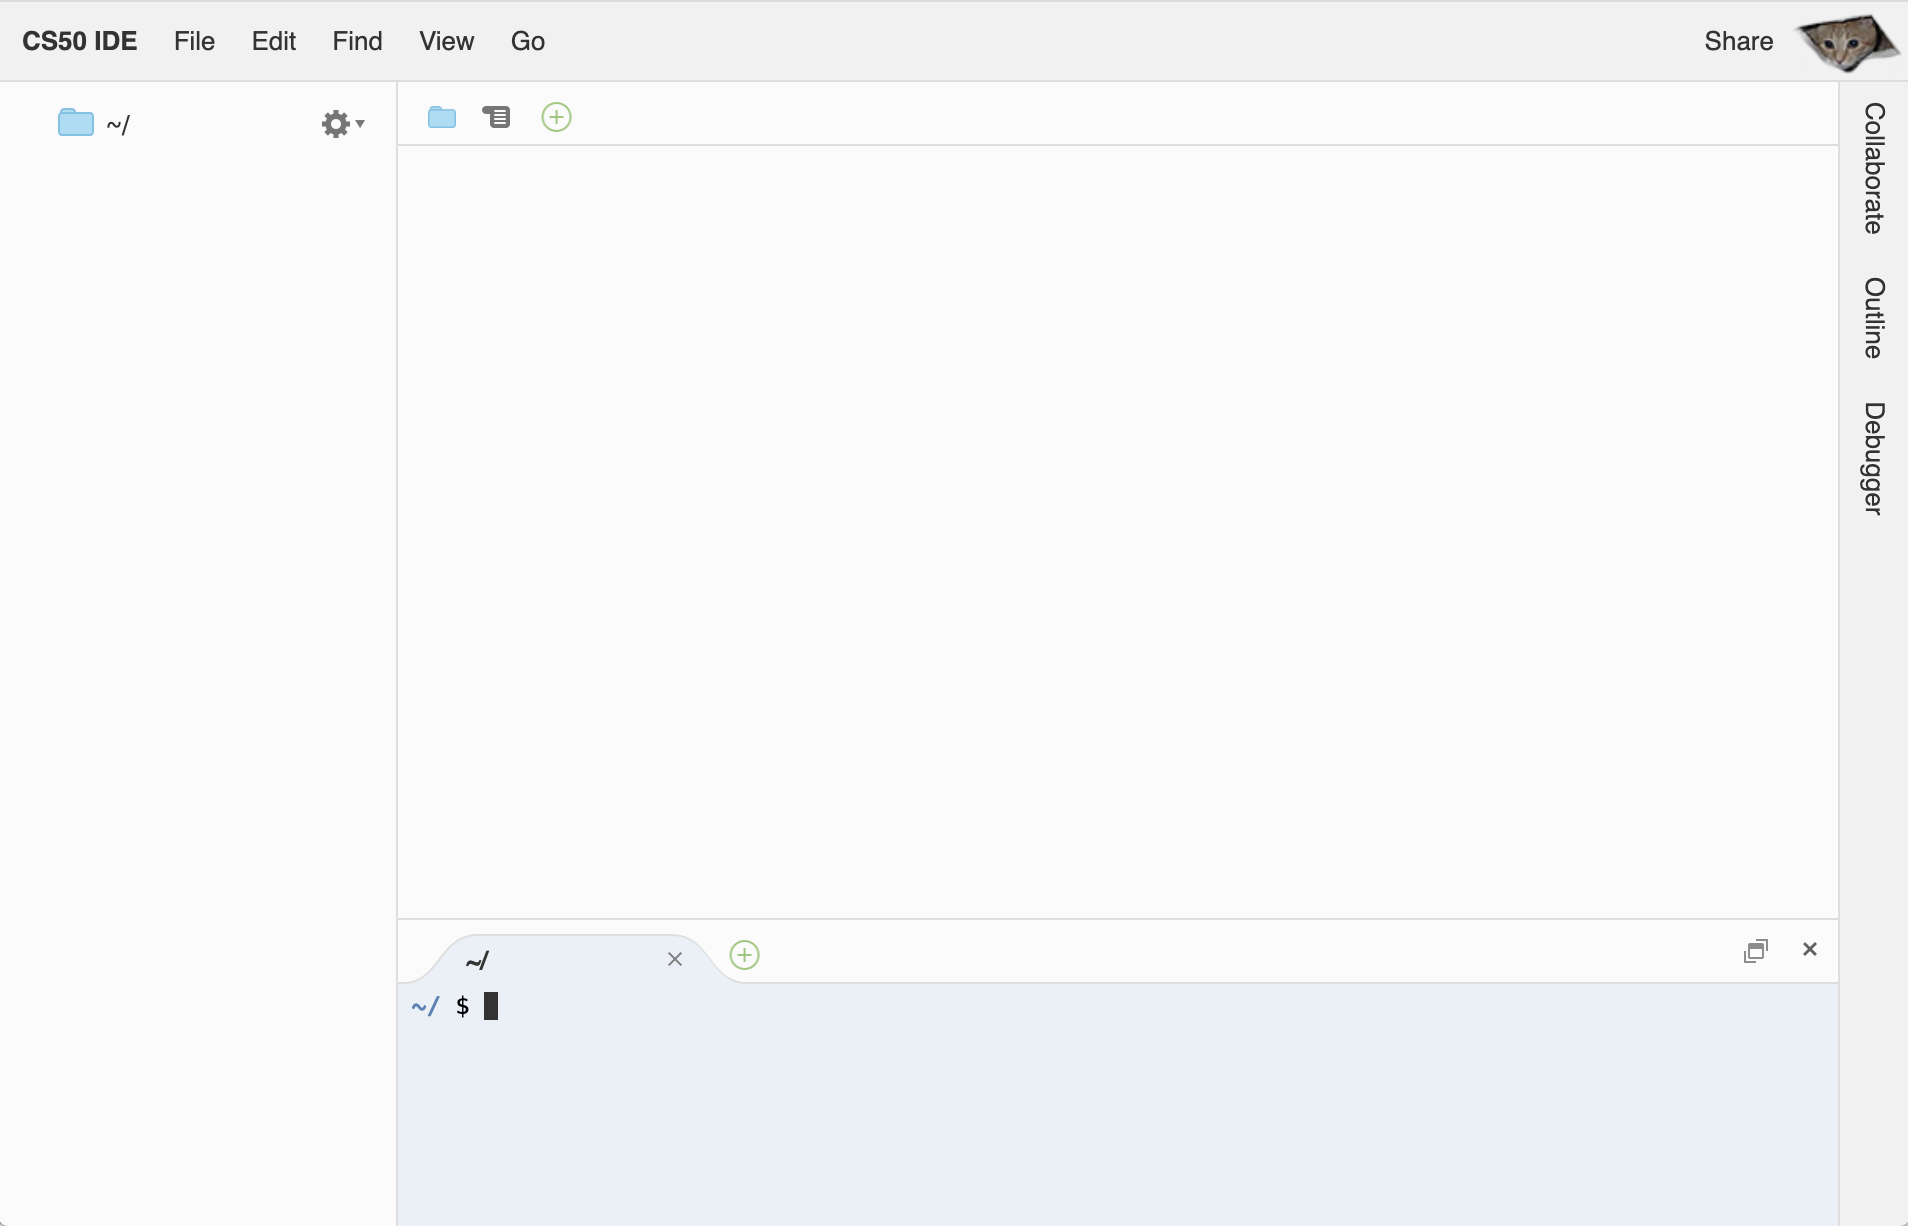
\includegraphics[scale=0.35]{img/cs50-clean}
\caption{CS50 IDE}
\end{figure}

First observe the major layout areas as depicted in Figure \ref{fig:cs50idehighlighted}.

\begin{enumerate}
  \item File Navigator - This is a graphical file explorer in which you can right click and create new directories (folders) and files, drag and drop to move things around, etc.
  \item File Editor - Double click on a plain text file and it will open in this file editor so you can edit it.  This is a tabbed environment so multiple files can be opened at once.
  \item Console - this is a Text User Interface (TUI) console in which you can type and execute commands to compile and run (text-based) programs in a Linux environment.
\end{enumerate}

\begin{figure}[h]
\centering
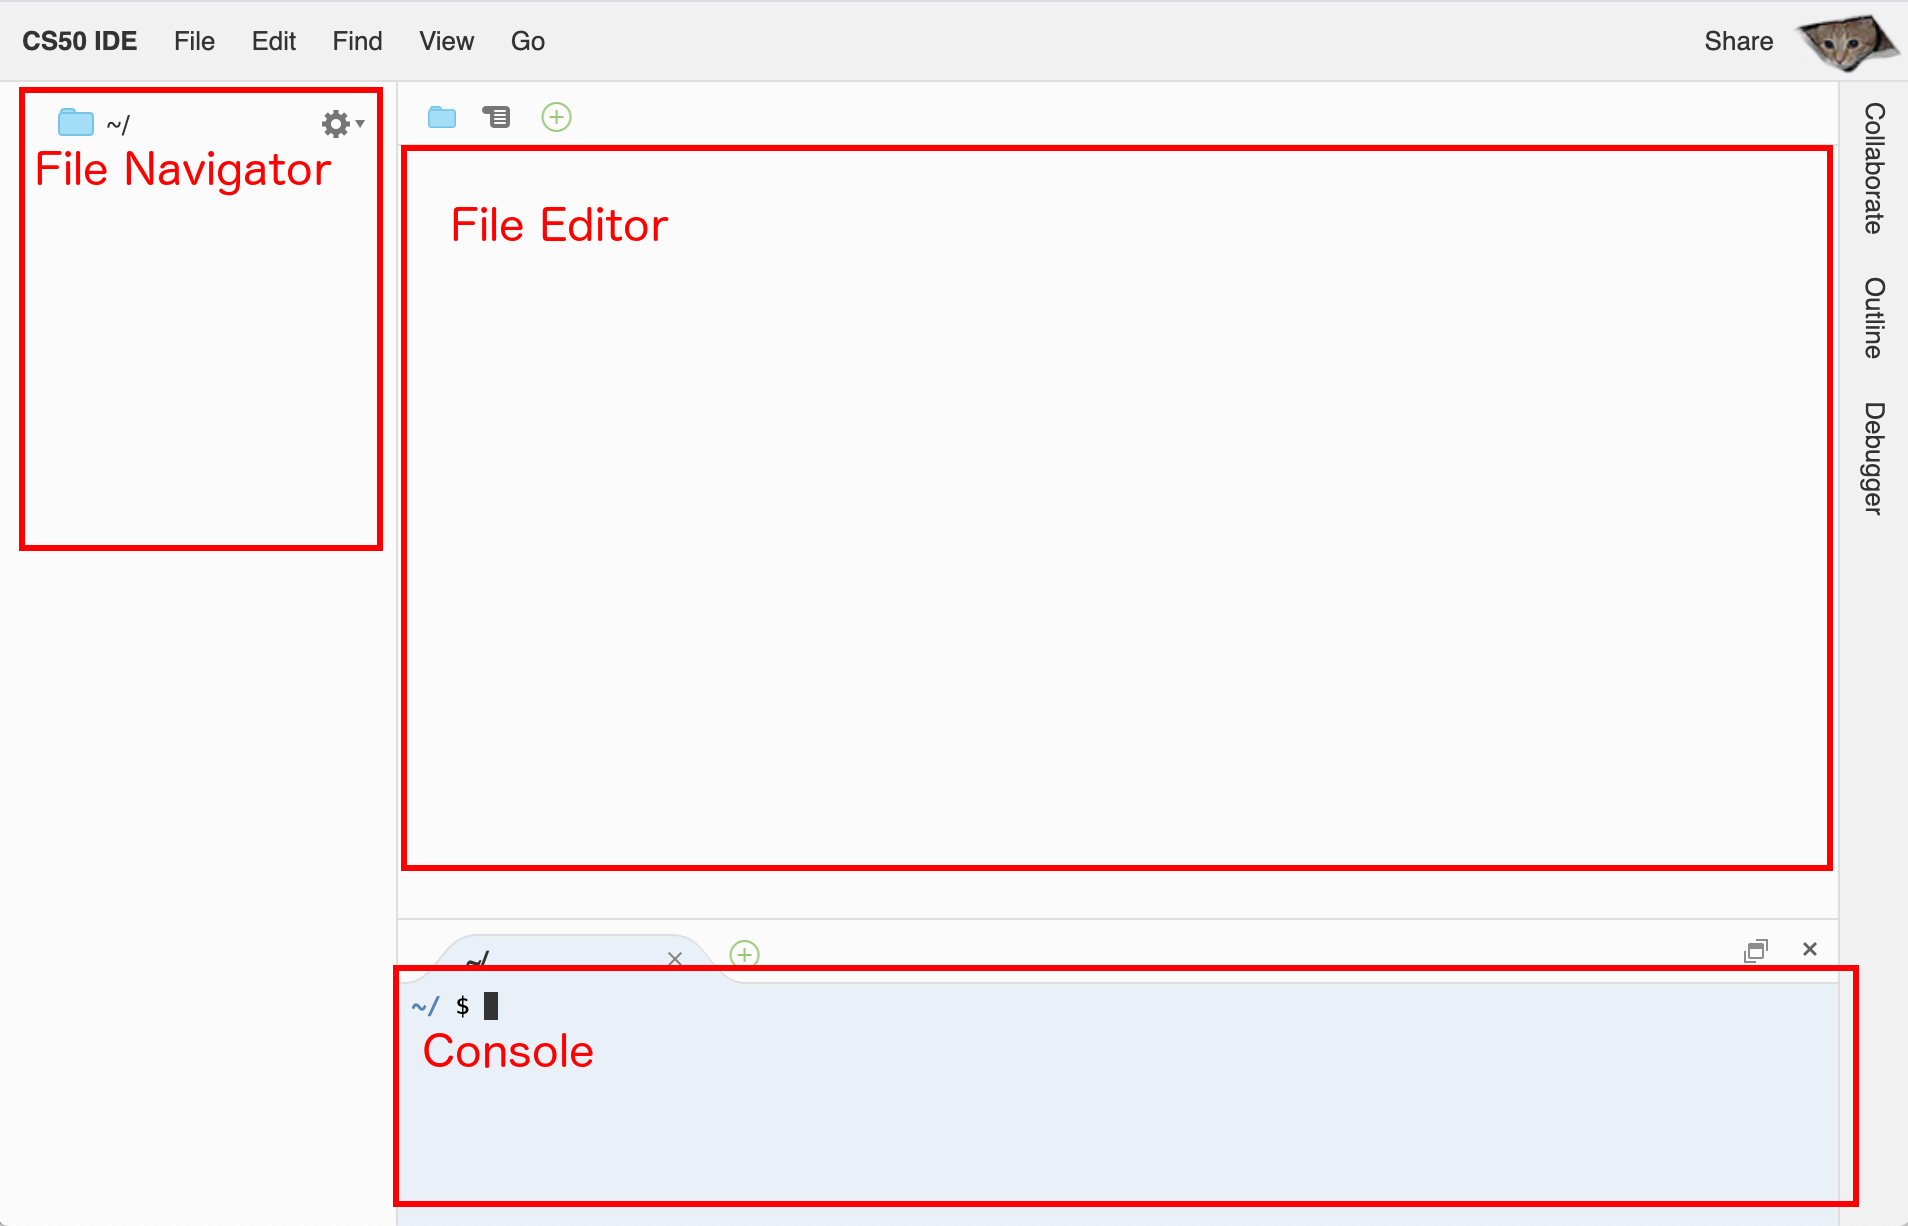
\includegraphics[scale=0.35]{img/cs50-highlighted}
\caption{CS50 IDE with layout sections highlighted}
\label{fig:cs50idehighlighted}
\end{figure}

Let's explore the basics:
\begin{enumerate}
  \item Create folders (right click the \emph{root} folder) named \mintinline{text}{labs} (in which we'll keep all our lab code, \mintinline{text}{hacks} (in which we'll do the same for hacks) and \mintinline{text}{misc}
  \item Create a file named \mintinline{text}{info.md} in the \mintinline{text}{misc} directory (again, right click the folder).  Double click the file and edit it (type your name and email).  Be sure to save.
  \item Now we'll get familiar with the console and some basic unix commands.  Click
  in the console area.  When we say type a command, we mean type the command and then
  hit enter to execute the command.
  \begin{enumerate}
    \item Type the command \mintinline{text}{ls} (short for ``list'') and 
    hit enter.  This lists the files and directories in the 
    \emph{current working directory}.  You should see your three directories.
    \item Let's change our current working directory so that we're \emph{in}
    the \mintinline{text}{misc} directory.  Type the following command
    \mintinline{text}{cd misc} (short for ``change directory'').  Type \mintinline{text}{ls} again and you'll see your \mintinline{text}{info.md} file.
    \item You can determine \emph{where} in the directory structure you are
    by typing the command \mintinline{text}{pwd}.  Try it; you'll see that your
    \mintinline{text}{misc} directory is actually under the \mintinline{text}{/home/ubuntu/} directory
    \item You can go back ``up'' the directory structure by typing the command
    \mintinline{text}{cd ..} (\mintinline{text}{..} is short hand for the \emph{parent} directory or one directory up in the hierarchy)
    \item You can also remove a file using the \mintinline{text}{rm fileName} 
    command which will \emph{permanently delete} the file.  Careful, there
    is no undo or recycle bin!  You can also remove a file by right clicking
    and deleting it in the File Navigator.
  \end{enumerate}
\end{enumerate}

%Before we go on, let's setup our environment for the rest of the semester.
%Type the following command (you may want to copy and paste) to install 
%several libraries:
%
%\begin{minted}{text}
%sudo apt-get install libcmocka-dev libcmocka0 cmocka-doc unixodbc 
%odbcinst gtk+-3.0 libcurl4-gnutls-dev -y
%\end{minted}

A more comprehensive tutorial on unix commands is available here: 
\url{http://www.math.utah.edu/lab/unix/unix-commands.html}.

\subsection{Editing Code}

Programming requires that you write code in a \emph{source file}, 
a plain text file that contains syntactically valid programming 
commands.  In general, you can use any plain text editor to edit
code (MS Word is not a plain text editor).  However, it is much
better to use a text editor designed for code that uses 
\emph{syntax highlighting} to help you differentiate various programming elements
by highlighting them in different colors and fonts.  The CS50 IDE
provides such an editor.  Let's practice writing some code.

\begin{enumerate}
  \item In your \mintinline{text}{misc} directory create a new file
  named \mintinline{text}{hello.c}
  \item Open the file and edit its contents to look like the 
  following but with your name and the current date.
  
\begin{minted}{c}
/**
 * Author: Your Name
 * Date: 20xx/xx/xx
 *
 * A simple hello world program in C
 *
 */
#include <stdlib.h>
#include <stdio.h>

int main(int argc, char **argv) {

  printf("Hello World!\n");

  return 0;
}
\end{minted}

  \item Save the file
  \item Now let's \emph{compile} this code into an executable program.
  In the console, type the following command (be sure you're still in the 
  \mintinline{text}{misc} directory): %Make this an intention mistake in the video

  \mintinline{text}{gcc hello.c}
  
  \mintinline{text}{gcc} (GNU Compiler Collection) is a C compiler.  
  In general in unix/linux if a command is successful nothing will 
  be displayed; ``no news is good news.''  If you made a mistake the
  compiler will give you a (sometimes) helpful hint about what was wrong.
  If you made a mistake fix it and repeat until it successfully compiles.
  \item When successful the compiler produces an \emph{executable} file 
  named \mintinline{text}{a.out}.  Use \mintinline{text}{ls} to verify 
  that the new file has been created (or observe it in the File Navigator).  
  \item Run your program by typing the following command: 
  \mintinline{text}{./a.out} which should print \mintinline{text}{Hello World!}
  to the Console.  
\end{enumerate}

Congratulations on your first program!

\subsection{Checking Out Code From Github}

Each lab will have some starter code and other \emph{artifacts} (data files, 
scripts, etc.) that will be provided to get you started.  The code is hosted
on GitHub (\url{https://github.com}) and you must \emph{clone} a copy of
it to your own workspace.

\begin{enumerate}
  \item Change your current working directory to your \mintinline{text}{labs}
  directory.  To do this you can use \mintinline{text}{cd ..} then 
  \mintinline{text}{cd labs} (assuming you are currently in \mintinline{text}{misc})
  or you can do this in one step: 
  
  \mintinline{text}{cd ../labs}
  
  which means ``go up one directory, then down to \mintinline{text}{labs}.''
  \item To clone, use the the following command:
  
  \mintinline{text}{git clone https://github.com/cbourke/CSCE155-C-Lab01}

  \item A new directory, \mintinline{text}{CSCE155-C-Lab01} should be created, 
  go into this directory by typing \mintinline{text}{cd CSCE155-C-Lab01}
  
  \item List the contents of this directory by typing \mintinline{text}{ls}.  
  If everything worked, there should be a \mintinline{text}{hello.c} 
  file in your directory similar to the one you just wrote.
\end{enumerate}

Boring.  Been there done that.  So, let's modify the program. 

\begin{enumerate}
  \item Open the \mintinline{text}{hello.c} source file (you now
  have two files with that name, so be sure you're editing the
  correct one or close the other).
  \item Modify the file by changing the author to you (and your 
  partner if you have one) and change the date.
  \item Change the message that is produced by the program (the
    \mintinline{c}{printf} statement) to instead
  	print you (and your partner's) name.
  \item Save, compile and run your program to make sure it works.
\end{enumerate}

\subsection{Submitting Your Program}

Many of your assignments will include a programming portion that will 
require you to hand in \emph{soft copy} source files for graders to compile 
and evaluate.  To do this, you will use a the CSE webhandin.

\begin{enumerate}
  \item First, we need to get your source file to \emph{your computer}.
  Right now, the files only exist on the CS50 IDE server.  Right click
  on the \mintinline{text}{hello.c} file and click download.  You
  can also download a copy of your entire project using File $\rightarrow$
  Download Project (in fact, it is a good idea to periodically backup
  your project by downloading it, but using git is a much better solution).
  \item Point a new browser tab to \url{https://cse-apps.unl.edu/handin}
  \item Login with your CSE credentials
  \item Click on this course and lab 01.  You can either click the 
  large ``handin'' area and select your downloaded \mintinline{text}{hello.c} 
  file or you can drag-drop the file.  You can (re)submit the same file as
  many times as you want up until the due date.  
\end{enumerate}

Some things to understand about webhandin:
\begin{itemize}
  \item File names are case sensitive and you may only submit files
  with names as specified by the particular assignment
  \item There is no need to delete the file if you need to resubmit 
  it, the old version will be overwritten
  \item If you make no changes to the file the resubmission will be rejected
  \item The most common mistake is handing in the \emph{wrong version}
  of a file, so be aware of which file(s) you're handing in
\end{itemize}

\subsection{Grading Your Program}

Now that the file has been handed in, you can ``grade'' yourself 
by using the webgrader.

\begin{enumerate}
  \item Open a new tab/window and point your browser to one of 
  the following depending on which course you are in:
  \begin{itemize}
    \item CSCE 155E: \url{https://cse.unl.edu/~cse155e/grade}
    \item CSCE 155H: \url{https://cse.unl.edu/~cse155h/grade}
    \item ECEN 1940: \url{https://cse.unl.edu/~c-ecen1940/grade}
  \end{itemize}
  \item Fill the form with your CSE login and password, select 
  the appropriate assignment (Lab 01), click ``Grade'' and
  observe the results.
\end{enumerate}

Some things to understand about webgrader:
\begin{itemize}
  \item For future assignments and labs, you can compare the results of 
  	your program with the ``Expected Results''.  In general, the output
	does not need to match \emph{exactly} as long as you report \emph{at least}
	as much information as the expected output, you're probably good.
  \item If there are problems or errors with your program(s), 
    you should fix/debug them and repeat the handin/grading process.
	You can do this as many times as you like up until the due date.  
  \item Some programs 
	and assignments will run test cases and may provide expected output alongside 
	your output.  Others may have more sophisticated test cases and actually provide 
	you a percentage of test cases passed.  It is your responsibility to read, 
	understand and \emph{address} all of the errors and/or warnings that the grader produces.
  \item The webgrader is a \emph{black box} tester meaning you don't have
  access to its internal workings.  You should properly and thoroughly test
  and debug your programs locally instead of relying on webgrader as a 
  ``blind tester''
\end{itemize}


\end{document}
